\subsection{Introduction}
The published $H\rightarrow WW\rightarrow 2\ell 2\nu$ analysis of 2010 was based on the following electron selection:
\begin{itemize}
\item identification: VBTF80;
\item isolation: relIso$<$0.10, where relIso is the sum of contributions from tracks, ECAL, and HCAL in a cone of R=0.3 around the electron, 
divided by the electron $p_T$; in the barrel the ECAL contribution has a pedestal subtraction of 1 GeV;
\item impact parameter: transverse longitudinal parameter w.r.t. the primary vertex $<0.02$ cm and longitudinal i.p. $<$ 0.2 cm;
\item conversion rejection: 0 missing inner expected hits and partner track veto (distance $<$0.02 cm, $\Delta \cot \theta <$0.02).
\end{itemize}
Before the 2011 data taking we wanted to review the selection and check if there is anything better available.

This process is divided into two steps: we review the available selections for high $p_T$ electrons ($>$20 GeV) and then, 
we look for improvement for a possible extension at low $p_T$.

The choice of the optimal selection is based on the analysis results after all cuts, 
but we cross-check the performance in terms of efficiency of fake vs good electrons.
Also, we checked the performance in 2011 data and with high PU conditions.

\subsection{Procedure Definition}
The performance of the tested algorithms are evaluated using three figures of merit (FOM):
\begin{itemize}
\item FOM1: $S/B$, the signal to background ratio;
\item FOM2: $S/\sqrt{S+B}$, the statistical significance;
\item FOM3: $S/\sqrt{S+B+(0.35 \cdot B)^2}$, the significance including a 35\% systematic uncertainty on the background;
\end{itemize}
where S and B are the total signal and background yields for an integrated luminosity of 1/fb and evaluated in the 2010 
$H\rightarrow WW\rightarrow 2\ell 2\nu$, $m_H=130$ GeV analysis signal region:
$\Delta\phi < 60$, 12$< m_{ll} <$45 GeV, projected Met$>$35 GeV (20 GeV for $\mu$-e final state), jet and top veto.
In this exercise we consider the final states where the trailing lepton is an electron ($\mu$-e and e-e).
The choice of 35\% in the FOM3 definition is somewhat arbitrary; the idea is to pick a conservative value on the background systematic uncertainty, 
as opposed to FOM2 where the assumption of negligible systematic uncertainty is too optimistic.

Yields are evaluated according to a simple model that treats good and fake electrons separately.
Real electrons are well modeled by simulation and thus we can rely on efficiency estimates from Monte Carlo; 
we use the electron efficiency from the signal sample to scale the signal and non-fake background yields.
Fake and non-prompt electrons, instead, can't be studied on simulation since their physics origin is difficult to parametrize and because
the available sample has low statistics. 
Therefore, we predict the fake background yield from data with the following procedure: 
first, we take as baseline the prediction from 2010 data scaled to 1/fb (using the fake rate method for 2010 analysis electron selection); 
then for each of the tested selections, we calculate the efficiency per fake electron from data and use this efficiency to scale the baseline prediction.

Fake electrons from data are selected from the EG2010A sample requiring HLT\_Ele10\_SW\_L1R and rejecting electrons from W and Z with the following cuts:
Met$<$20 GeV, $m_T(e, Met)<$20 GeV and, for event with two electrons, $|m_{ee}-m_Z|>$15 GeV. 
The selected sample includes about 6500 electrons passing the 2010 analysis selection.

Yields and efficiencies are computed in three bins both in $p_T$ ($[10,15],[15,20],[20,\infty]$, values in GeV) 
and in $|\eta|$ ($[0,1.0],[1.0,1.5],[1.5,2.5]$). 
Tables~\ref{tab:fakeBaseline}-\ref{tab:hww130yieds} report the baseline prediction from 2010 fake data and non-fake background and signal from MC.
For 10$<p_T<$15 GeV the background contribution from fakes is dominant, while at higher $p_T$ it is comparable or smaller than the sum of the other backgrounds.

\begin{table}[!ht]
\begin{center}
\begin{tabular}{|c|ccc|c|} \hline
 & $0.0<|\eta|<1.0$ & $1.0<|\eta|<1.5$ & $1.5<|\eta|<2.5$ & All $\eta$ \\ \hline
10$<p_T<$15 & 9.11 & 3.41 & 1.18 & 13.70 \\
15$<p_T<$20 & 3.22 & 0.00 & 0.93 & 4.15 \\
$p_T>$20 & 1.24 & 2.85 & 1.05 & 5.14 \\  \hline
All $p_T$ & 13.57 & 6.26 & 3.16 & 22.99 \\ \hline
\end{tabular}
\caption{Fake rate prediction for $\mu$-e and e-e final states from 2010 data. 
The electron selection is the same as in 2010 analysis and the results is scaled to 1/fb.
The total uncertainty is of the order of 50\%.
\label{tab:fakeBaseline}}
\end{center}
\end{table}

\begin{table}[!ht]
\begin{center}
\begin{tabular}{|c|ccc|c|} \hline
 & $0.0<|\eta|<1.0$ & $1.0<|\eta|<1.5$ & $1.5<|\eta|<2.5$ & All $\eta$ \\ \hline
10$<p_T<$15 & 2.15 & 0.81 & 1.03 & 4.00 \\
15$<p_T<$20 & 4.18 & 1.42 & 1.26 & 6.87 \\
$p_T>$20    & 10.26& 4.89 & 3.57 & 18.71\\  \hline
All $p_T$   & 16.59& 7.12 & 5.86 & 29.58 \\ \hline
\end{tabular}
\caption{MC yield prediction for non-fake electron backgrounds ($\mu$-e and e-e final states). 
The electron selection is the same as in 2010 analysis and the results is scaled to 1/fb.
\label{tab:nonfakeyieds}}
\end{center}
\end{table}

\begin{table}[!ht]
\begin{center}
\begin{tabular}{|c|ccc|c|} \hline
 & $0.0<|\eta|<1.0$ & $1.0<|\eta|<1.5$ & $1.5<|\eta|<2.5$ & All $\eta$ \\ \hline
10$<p_T<$15 & 0.79 & 0.22 & 0.18 & 1.19 \\
15$<p_T<$20 & 1.09 & 0.37 & 0.32 & 1.78 \\
$p_T>$20    & 2.18 & 0.69 & 0.54 & 3.41 \\  \hline
All $p_T$   & 4.06 & 1.28 & 1.04 & 6.38 \\ \hline
\end{tabular}
\caption{MC yield prediction for $H\rightarrow WW$ sample ($m_H=130$ GeV) ($\mu$-e and e-e final states). 
The electron selection is the same as in 2010 analysis and the results is scaled to 1/fb.
\label{tab:hww130yieds}}
\end{center}
\end{table}

We optimize the electron identification, isolation and impact parameter selections separately, changing one cut at a time.
We checked that, using different isolation algorithms as baseline, the optimal identification working point is the same.
Therefore, we use the 2010 selection as a baseline for the optimization process.

\subsection{Electron Identification}

We compared the performance of several electron identification algorithms available in the collaboration.
They can be grouped in three sets:
\begin{itemize}
\item Simple Cuts (VBTF: 4 variables, separate cuts for barrel/endcap): 
  \begin{itemize}
  \item VBTF85
  \item VBTF80 
  \item VBTF70
  \end{itemize}
\item Multivariate techniques, exploiting correlations between variables (MVA): 
  \begin{itemize}
  \item MVA05: particle flow MVA output$>$0.5 
  \item MVA07: particle flow MVA output$>$0.7 
  \item LHT: Likelihood ID, tight WP\footnote{UserCode/emanuele/EgammaAnalysisTools, tag ``edm-Feb2011'' and latest PDFs: \\
http://indico.cern.ch/getFile.py/access?contribId=4\&resId=0\&materialId=slides\&confId=127254.}
  \end{itemize}
\item Categorized cuts (CIC: advanced cut based tuning in multiple categories)\footnote{CIC version V06 with data driven tuning \\
http://cmssw.cvs.cern.ch/cgi-bin/cmssw.cgi/CMSSW/RecoEgamma/ElectronIdentification/python/\\
cutsInCategoriesElectronIdentificationV06\_DataTuning\_cfi.py?view=log.}: 
  \begin{itemize}
  \item CICST: CIC SuperTight ID 
  \item CICHT2: CIC HyperTight v2 ID
  \item CICHT4: CIC HyperTight v4 ID
  \end{itemize}
\end{itemize}

\subsubsection{Results for $p_T>$20 $\GeVc$}

The first step is the definition of a baseline cut at high $p_T$. 
We verify the identification performance by comparing the cut efficiency on fake electrons from data and on signal electrons on MC.
Figure~\ref{subfig:idEffic_gt20} shows that the MVA curve has worse rejection power than CIC, while the VBTF and CIC curves cross.
This result can be interpreted in terms of analysis performance by looking at the FOM's for $p_{T,max}>$20 GeV and $p_{T,min}>$20 GeV
(Figs.~\ref{subfig:id_hww130_fom1_pt20}-\ref{subfig:id_hww130_fom3_pt20}). 
No algorithm provides the best results for all FOM's; however, it is clear that MVA is slightly worse, while VBTF and CIC are comparable.
Therefore, we think that it is safe to continue with the VBTF approach as baseline for the analysis:
reasonable working points for the $m_H=$130 GeV analysis are VBTF80 and VBTF70. 
However, VBTF70 might be too tight for mass values higher than $m_H=$130 GeV where the $p_T$ spectrum of the signal leptons 
is harder and the fake background less important.
 
\begin{figure}[!hbtp]
\subfigure[]{
\centering
\label{subfig:idEffic_gt20}
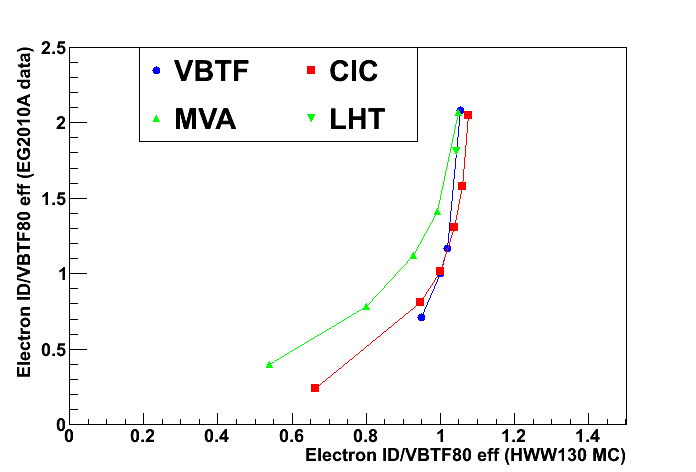
\includegraphics[width=.45\textwidth]{figures/idEffic_gt20.png}}
\subfigure[]{
\centering
\label{subfig:id_hww130_fom1_pt20}
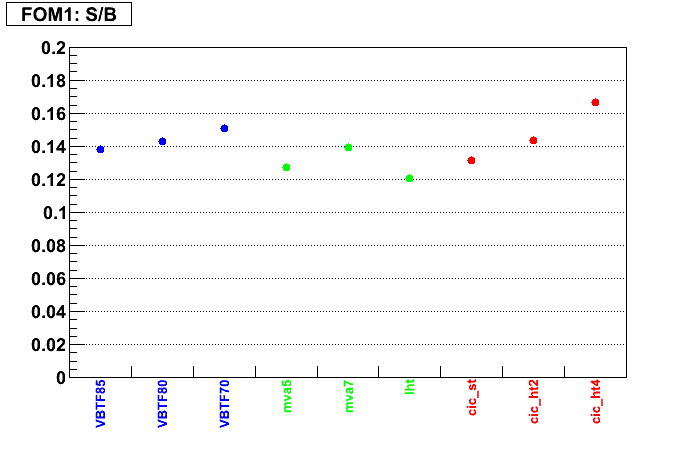
\includegraphics[width=.45\textwidth]{figures/id_hww130_fom1_pt20.png}}\\
\subfigure[]{
\centering
\label{subfig:id_hww130_fom2_pt20}
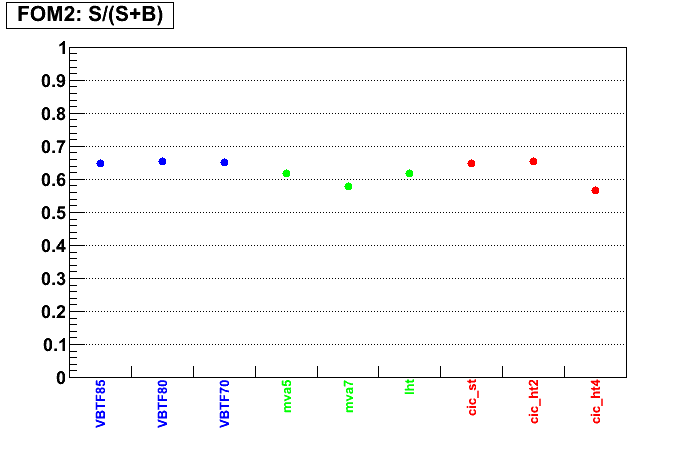
\includegraphics[width=.45\textwidth]{figures/id_hww130_fom2_pt20.png}}
\subfigure[]{
\centering
\label{subfig:id_hww130_fom3_pt20}
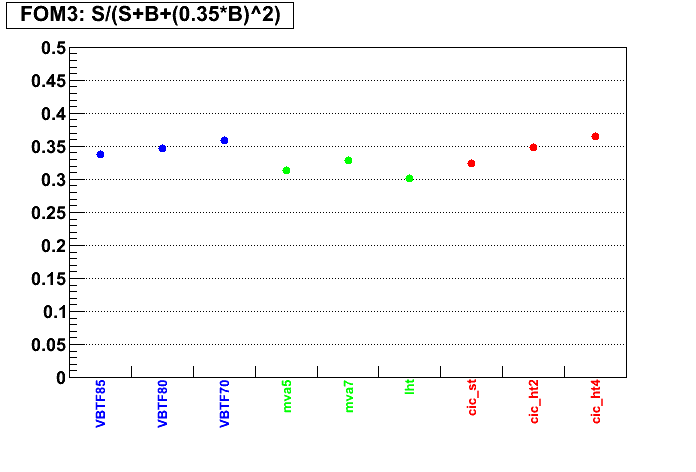
\includegraphics[width=.45\textwidth]{figures/id_hww130_fom3_pt20.png}}\\
\caption{Relative ID efficiency (w.r.t. VBTF80) on fake electrons from data vs good electrons from signal MC \subref{subfig:idEffic_gt20};
FOM1, FOM2 and FOM3 \subref{subfig:id_hww130_fom1_pt20},\subref{subfig:id_hww130_fom2_pt20},\subref{subfig:id_hww130_fom3_pt20}. 
Electrons have $p_T>$20 GeV; the 2010 selection is used as a baseline, the ID cut is varied only.}
\label{fig:idpt20}
\end{figure}

\subsubsection{Additional Requirements for $p_T<$20 $\GeVc$}

The cut based approach is a reasonable choice as a baseline for high $p_T$, but at low $p_T$ fakes dominate and more rejection power might be needed; 
Therefore, we propose an additional cut to tighten the selection at low $p_T$.

The idea is to introduce a simple categorization based on fbrem, $\eta$ and $E/p$ (Figure~\ref{fig:smurfcuts}).
When a particle passing electron ID criteria has a high fbrem (fbrem$>$0.15) we are confident it is an electron and we keep it;
the fake electron sample, instead, is dominated by low fbrem candidates.
Because of the high tracker material budget, at $|\eta|>$1 almost all signal electron radiate and thus we reject all electron candidates with fbrem$<$0.15.
At $|\eta|<$1, instead, there is less tracker material and electrons with low fbrem are frequent: in this region we keep electrons with $E/p>$0.95.

In summary, we apply the following additional cut for electrons with $p_T<$20 GeV:
\begin{equation}
fbrem>0.15~OR~(|\eta|<1~AND~E/p>0.95)
\end{equation}
In the following, we call VBTF80+ (VBTF70+) the VBTF80 (VBTF70) selection added of the proposed cut above.

\begin{figure}[!hbtp]
\subfigure[]{
\centering
\label{subfig:Data_fbrem_eta}
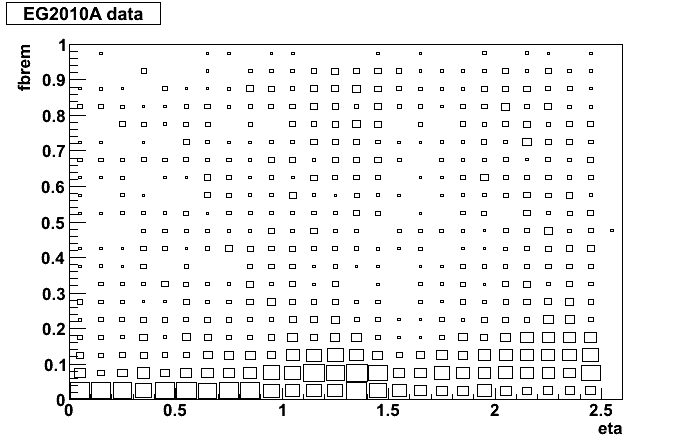
\includegraphics[width=.45\textwidth]{figures/Data_fbrem_eta.png}}
\subfigure[]{
\centering
\label{subfig:Data_eOverPIn_bar}
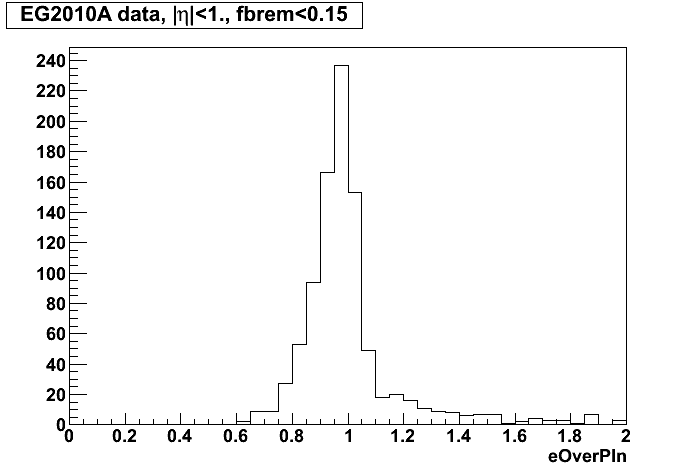
\includegraphics[width=.45\textwidth]{figures/Data_eOverPIn_bar.png}}\\
\subfigure[]{
\centering
\label{subfig:HWW130_fbrem_eta}
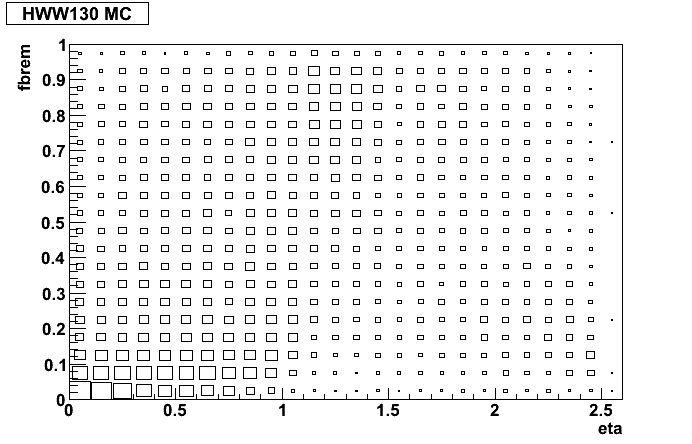
\includegraphics[width=.45\textwidth]{figures/HWW130_fbrem_eta.png}}
\subfigure[]{
\centering
\label{subfig:HWW130_eOverPIn_bar}
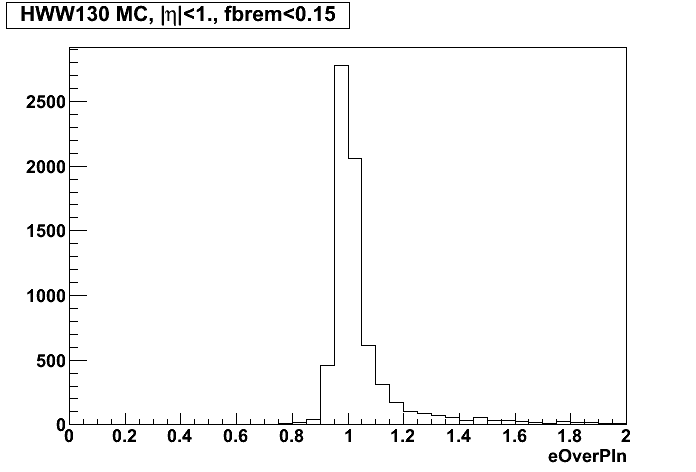
\includegraphics[width=.45\textwidth]{figures/HWW130_eOverPIn_bar.png}}\\
\caption{fbrem vs $|\eta|$ (left) and $E/p$ (right) distributions for fake electrons in data (up) and good electrons in signal MC (down).}
\label{fig:smurfcuts}
\end{figure}

\subsubsection{Results for 15$<p_T<$20 $\GeVc$}

The efficiency plot (Figure~\ref{subfig:idEffic_15pt20}) shows that, also in this $p_T$ range, the CIC curve is better than MVA and
the VBTF curve again goes across. It is worth noting that the kink in the last two points of the VBTF curve is due to the additional cuts.
The FOM's for $p_{T,max}>$20 GeV and $p_{T,min}>$15 GeV are shown in Figs.~\ref{subfig:id_hww130_fom1_pt15}-\ref{subfig:id_hww130_fom3_pt15}:
all FOM's are improved w.r.t. to the corresponding values for $p_{T,min}>$20 GeV and an additional improvement is gained using VBTF+.

\begin{figure}[!hbtp]
\subfigure[]{
\centering
\label{subfig:idEffic_15pt20}
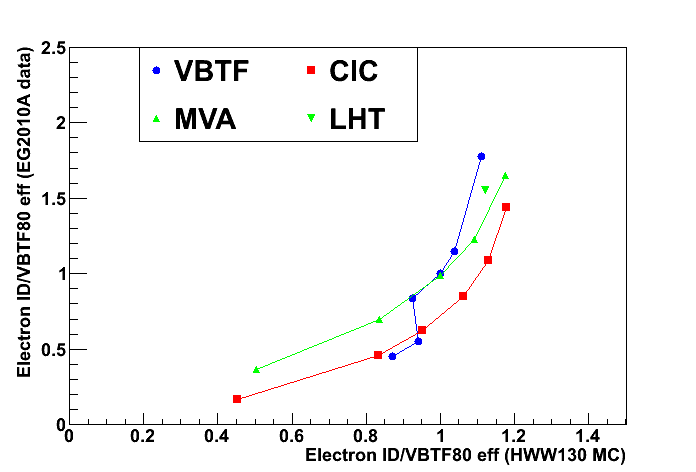
\includegraphics[width=.45\textwidth]{figures/idEffic_15pt20.png}}
\subfigure[]{
\centering
\label{subfig:id_hww130_fom1_pt15}
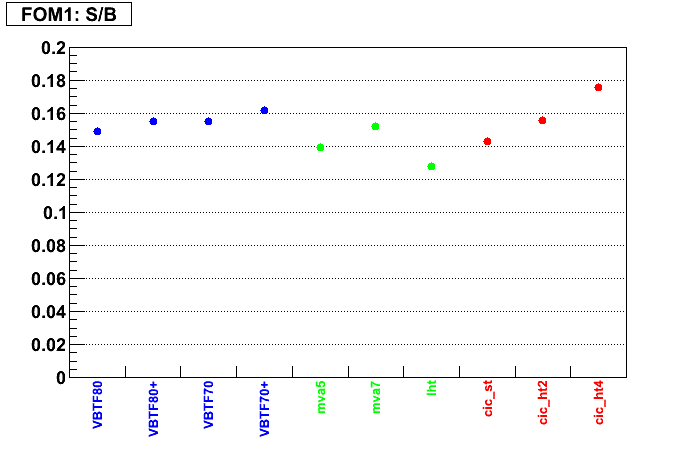
\includegraphics[width=.45\textwidth]{figures/id_hww130_fom1_pt15.png}}\\
\subfigure[]{
\centering
\label{subfig:id_hww130_fom2_pt15}
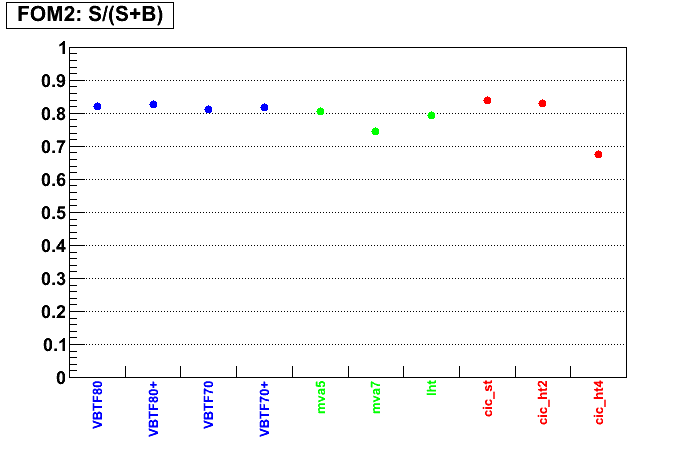
\includegraphics[width=.45\textwidth]{figures/id_hww130_fom2_pt15.png}}
\subfigure[]{
\centering
\label{subfig:id_hww130_fom3_pt15}
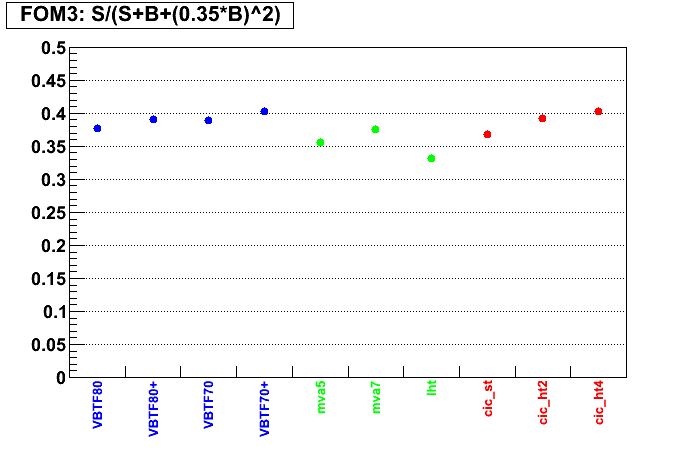
\includegraphics[width=.45\textwidth]{figures/id_hww130_fom3_pt15.png}}\\
\caption{Relative ID efficiency (w.r.t. VBTF80) on fake electrons from data vs good electrons from signal MC \subref{subfig:idEffic_15pt20} 
(15$<p_T<$20 GeV);
FOM1, FOM2 and FOM3 \subref{subfig:id_hww130_fom1_pt15},\subref{subfig:id_hww130_fom2_pt15},\subref{subfig:id_hww130_fom3_pt15} for analysis with  
$p_{T,min}>$15 GeV; the 2010 selection is used as a baseline, the ID cut is varied only.}
\label{fig:idpt15}
\end{figure}

\subsubsection{Results for 10$<p_T<$15 $\GeVc$}

Again, the VBTF+ cuts significantly improve the ID performance (Figure~\ref{subfig:idEffic_10pt15}).
However, despite VBTF+ brings a large relative improvement, because of the large amount of fakes in this region the FOM's 
(Figs.~\ref{subfig:id_hww130_fom1_pt10}-\ref{subfig:id_hww130_fom3_pt10}) do not show an overall enhancement w.r.t. $p_{T,min}>$15 GeV.

\begin{figure}[!hbtp]
\subfigure[]{
\centering
\label{subfig:idEffic_10pt15}
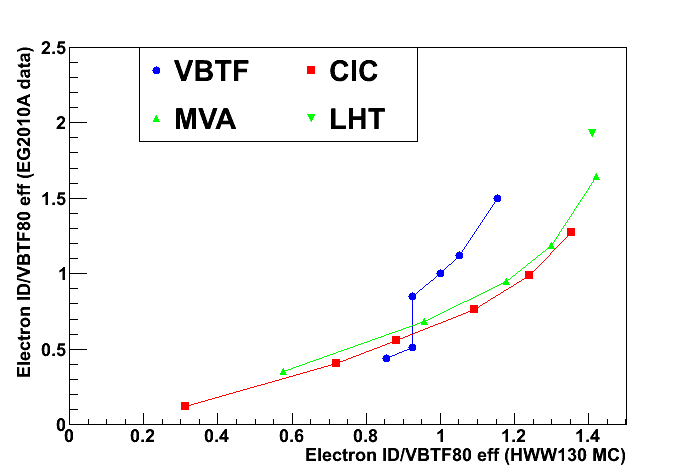
\includegraphics[width=.45\textwidth]{figures/idEffic_10pt15.png}}
\subfigure[]{
\centering
\label{subfig:id_hww130_fom1_pt10}
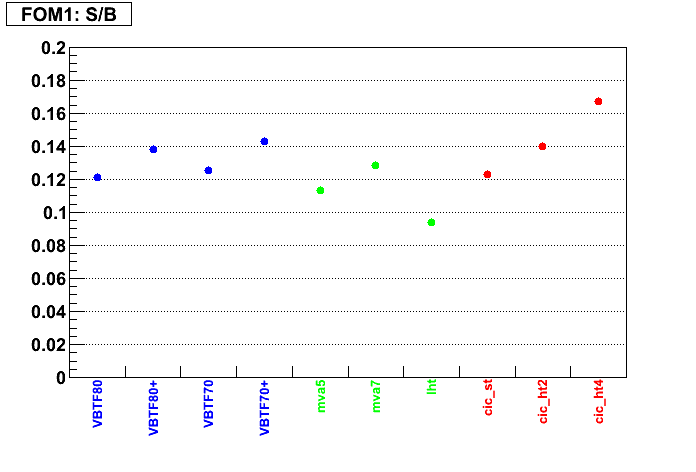
\includegraphics[width=.45\textwidth]{figures/id_hww130_fom1_pt10.png}}\\
\subfigure[]{
\centering
\label{subfig:id_hww130_fom2_pt10}
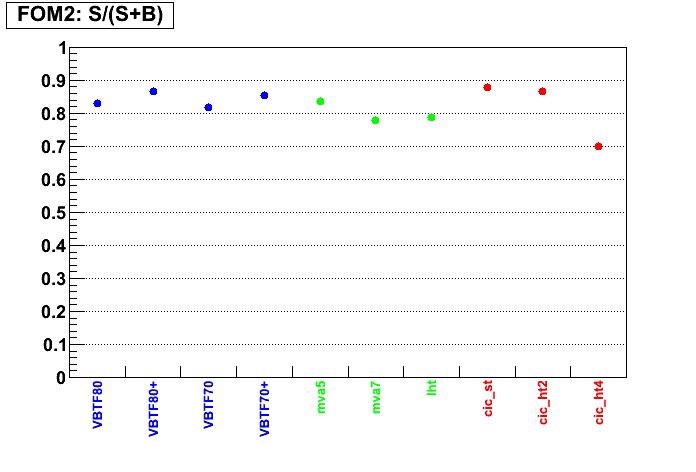
\includegraphics[width=.45\textwidth]{figures/id_hww130_fom2_pt10.png}}
\subfigure[]{
\centering
\label{subfig:id_hww130_fom3_pt10}
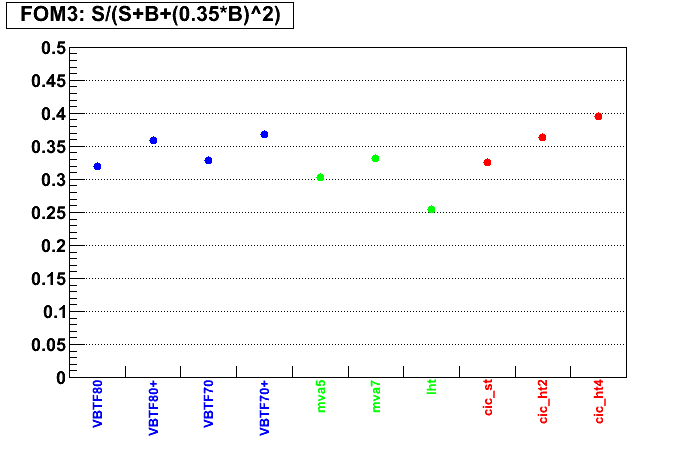
\includegraphics[width=.45\textwidth]{figures/id_hww130_fom3_pt10.png}}\\
\caption{Relative ID efficiency (w.r.t. VBTF80) on fake electrons from data vs good electrons from signal MC \subref{subfig:idEffic_10pt15} 
(10$<p_T<$15 GeV);
FOM1, FOM2 and FOM3 \subref{subfig:id_hww130_fom1_pt10},\subref{subfig:id_hww130_fom2_pt10},\subref{subfig:id_hww130_fom3_pt10} for analysis with  
$p_{T,min}>$10 GeV; the 2010 selection is used as a baseline, the ID cut is varied only.}
\label{fig:idpt10}
\end{figure}

\subsubsection{Conclusions}

In summary, the cut based approach for electron ID is optimal for the $H\rightarrow WW$ analysis and the proposed additional cuts add more rejection power 
for $p_T<$20 GeV. Lowering the $p_{T,min}$ cut to 15 GeV improves the analysis, while at 10 GeV there is no clear benefit. 
Thus, we choose VBTF80 for $p_T>$20 GeV and VBTF70+ for 15$<p_T<$20 GeV.

\subsection{Electron Isolation}

The 2010 analysis used relIso$<$0.10.
Given that the ID optimization suggests to lower the  $p_{T,min}$ cut to 15 GeV, we wanted to review if tightening the isolation cut further 
would improve the performance of the analysis.
Within the cut based approach, we can tighten the cut in three ways: lowering the cut value, increasing the cone size, and removing the pedestal subtraction.
In the following tests, we call (tight) sliding isolation the following set of cuts: 
\begin{itemize}
\item relIso$<$0.1 (0.1) for $p_T>$20 GeV
\item relIso$<$0.07 (0.03) for 15$<p_T<$20 GeV
\item relIso$<$0.05 (0.01) for 10$<p_T<$15 GeV
\end{itemize}
and we will test it with cone size 0.3 and cone size 0.4 with and without pedestal subtraction.
CIC isolation uses cone size 0.3 for the tracker and 0.4 for the calorimeters and does not apply pedestal subtracion; cut values are optimized for various categories.
Results are summarized in Figure~\ref{fig:isopt15}. 
The efficiency plot shows that the cut based approach is basically one single curve covering the whole range and it is slightly worse than CIC; 
however, there is not a clear advantage in using tighter isolation approaches since FOM1 and FOM3 slightly improve, while FOM2 worsens. 
Therefore, we choose to stick to the relIso$<$0.10 cut. This exercise will be repeated with 2011 fake data.

\begin{figure}[!hbtp]
\subfigure[]{
\centering
\label{subfig:isoEffic_15pt20}
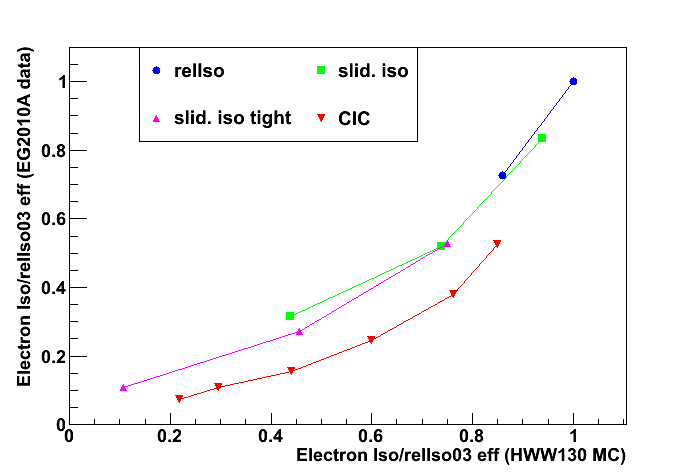
\includegraphics[width=.45\textwidth]{figures/isoEffic_15pt20.png}}
\subfigure[]{
\centering
\label{subfig:iso_hww130_fom1_pt15}
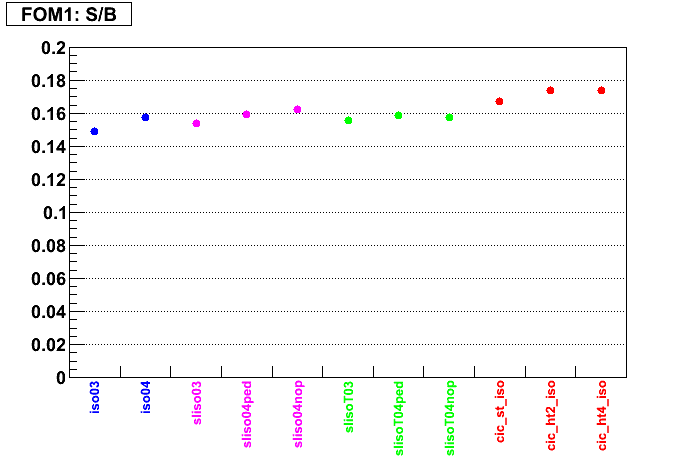
\includegraphics[width=.45\textwidth]{figures/iso_hww130_fom1_pt15.png}}\\
\subfigure[]{
\centering
\label{subfig:iso_hww130_fom2_pt15}
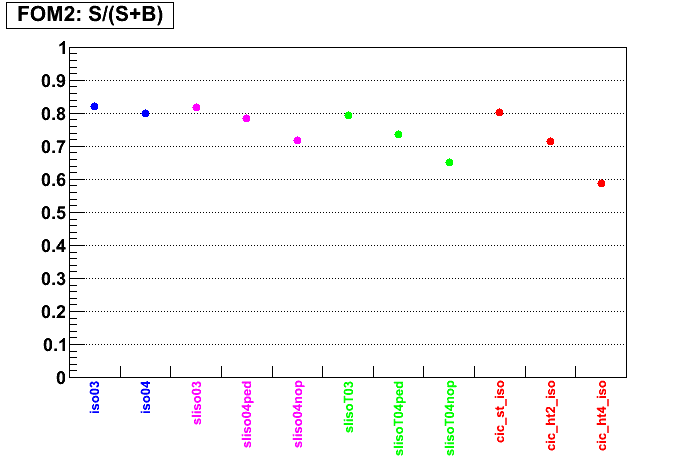
\includegraphics[width=.45\textwidth]{figures/iso_hww130_fom2_pt15.png}}
\subfigure[]{
\centering
\label{subfig:iso_hww130_fom3_pt15}
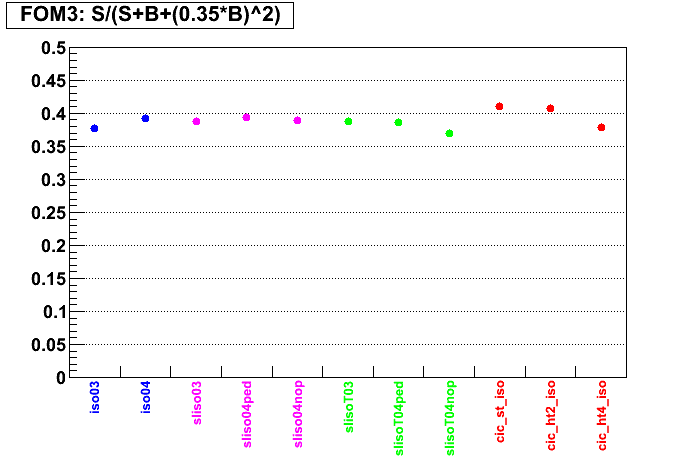
\includegraphics[width=.45\textwidth]{figures/iso_hww130_fom3_pt15.png}}\\
\caption{Relative isolation efficiency (w.r.t. relIso) on fake electrons from data vs good electrons from signal MC \subref{subfig:isoEffic_15pt20} 
(15$<p_T<$20 GeV);
FOM1, FOM2 and FOM3 \subref{subfig:iso_hww130_fom1_pt15},\subref{subfig:iso_hww130_fom2_pt15},\subref{subfig:iso_hww130_fom3_pt15} for analysis with  
$p_{T,min}>$15 GeV; the 2010 selection is used as a baseline, the isolation cut is varied only.}
\label{fig:isopt15}
\end{figure}

\subsection{Impact Parameter}

The same test have been performed varying the impact parameter (IP) cut.
We have tested the folowing approaches:
\begin{itemize}
\item 2D impact parameter cut
\item 2D impact parameter significance cut
\item 3D impact parameter cut
\item 3D impact parameter significance cut
\end{itemize}
where the impact parameter is computed with respect to the signal primary vertex (PV) reconstructed with the standard vertexing 
algorithm (\emph{offlinePrimaryVertex}).
Figure~\ref{subfig:ipEffic_15pt20} shows that, for 15$<p_T<$20 the best performance are obtained with the 2D impact parameter plain cut.
The FOM's show very little difference between the various approaches (Figs.~\ref{fig:ippt15}\subref{subfig:ip_hww130_fom1_pt15}-\subref{subfig:ip_hww130_fom3_pt15}).
We choose a 2D impact parameter cut value of 0.02 cm.

\begin{figure}[!hbtp]
\subfigure[]{
\centering
\label{subfig:ipEffic_15pt20}
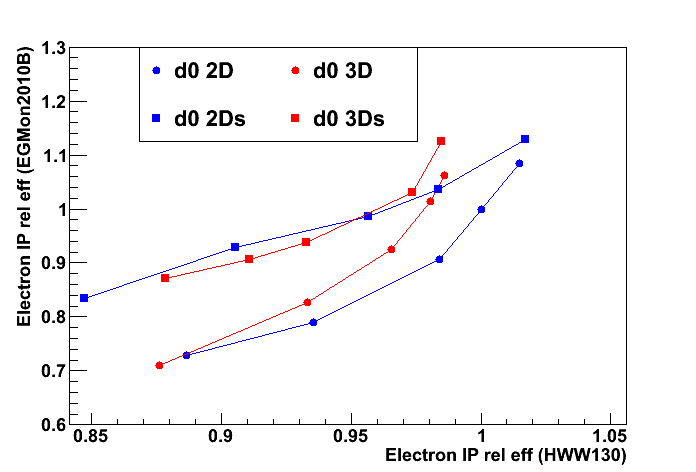
\includegraphics[width=.45\textwidth]{figures/ipEffic_lt20.png}}
\subfigure[]{
\centering
\label{subfig:ip_hww130_fom1_pt15}
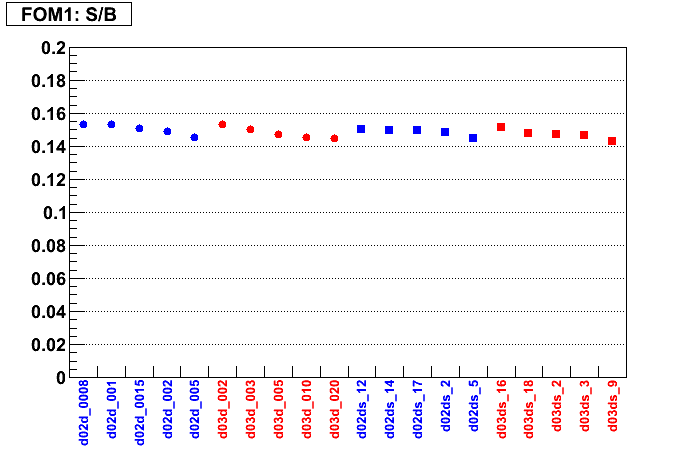
\includegraphics[width=.45\textwidth]{figures/ip_hww130_fom1_pt15.png}}\\
\subfigure[]{
\centering
\label{subfig:ip_hww130_fom2_pt15}
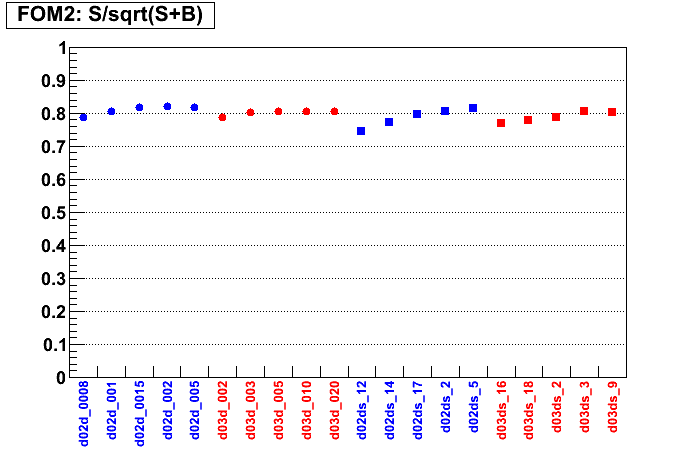
\includegraphics[width=.45\textwidth]{figures/ip_hww130_fom2_pt15.png}}
\subfigure[]{
\centering
\label{subfig:ip_hww130_fom3_pt15}
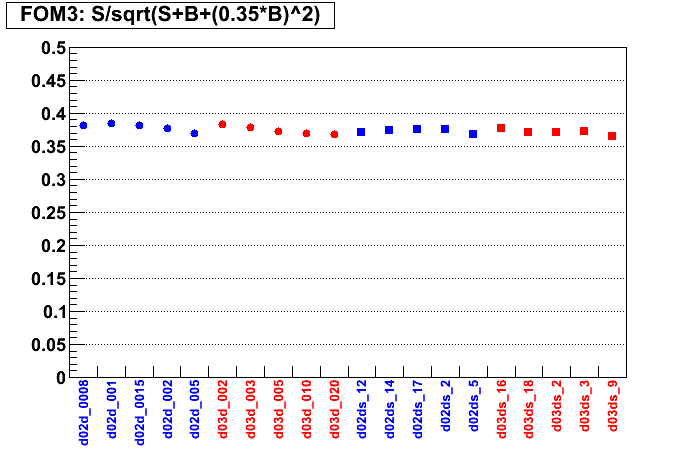
\includegraphics[width=.45\textwidth]{figures/ip_hww130_fom3_pt15.png}}\\
\caption{Relative IP efficiency (w.r.t. d0(PV)$<$0.02) on fake electrons from data vs good electrons from signal MC \subref{subfig:ipEffic_15pt20} 
(15$<p_T<$20 GeV);
FOM1, FOM2 and FOM3 \subref{subfig:ip_hww130_fom1_pt15},\subref{subfig:ip_hww130_fom2_pt15},\subref{subfig:ip_hww130_fom3_pt15} for analysis with  
$p_{T,min}>$15 GeV; the 2010 selection is used as a baseline, the d0 cut is varied only.}
\label{fig:ippt15}
\end{figure}

\subsection{Studies with Data}

We measured the efficiency of the additional proposed cuts on 2010 data using the tag and probe method.
We use a N-1 approach, where we choose di-electron events with 76$<M_{ee}<$106 GeV and the denominator is given by electrons passing 2010 analysis selection
and the numerator by 2010 selection plus the additional proposed cut. 
Results (Fig.~\ref{fig:eID-tnp}) show that the efficiency on Z electron is at the level of 90\%
or higher and data and MC are in good agreement. The error bars are statistical only.

\begin{figure}[!hbtp]
\centering
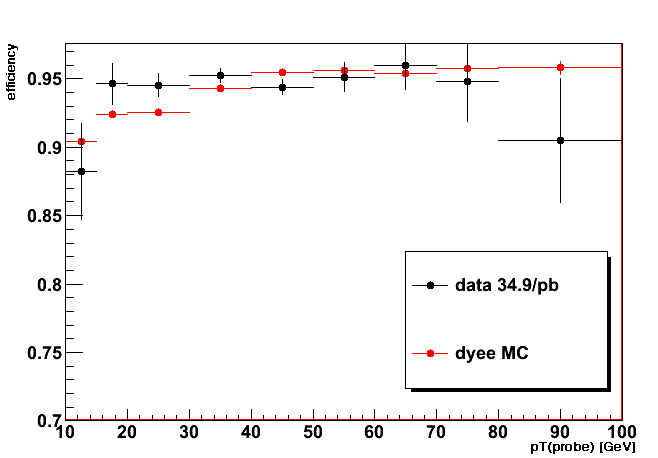
\includegraphics[width=.45\textwidth]{figures/eID-tnp.png}
\caption{Efficiency of the additional cut with the tag and probe method on 2010 $Z\rightarrow ee$ data and MC as a function of probe $p_T$.}
\label{fig:eID-tnp}
\end{figure}

We also checked the distribution of the electron ID variables in the first 2011 data and compared it with MC.
We analyzed ExpressStream data, selecting Z events with 76$<M_{ee}<$106 GeV, $p_{T,max}>$27 GeV (so that it passes the single electron trigger), 
$p_{T,min}>$10 GeV, relative isolation$<$0.2 for tracks, ECAL and HCAL separately and $\sigma_{i\eta i\eta}<$0.015 (0.031) for barrel (endcap).
Given that no selection for good run certification is applied, all distributions (Figs.~\ref{fig:mcdata_vbtf_bar}-\ref{fig:mcdata_smurf}) 
are in reasonable agreement except $H/E$ in the endcap (Fig.~\ref{subfig:mcdata_hOverE_end_log}). 
As other studies on high pile-up samples confirm, this variable is particularly sensitive to the pile-up conditions and can introduce data-MC discrepancies 
in the electron identification efficiency up to the 20\% level at large $|\eta|$.
We verified that with our current selection (VBTF80 for $p_T>$20 GeV and VBTF70+ for 15$<p_T<$20 GeV) we can remove the $H/E$ cut in the endcap
region without significant decrease in the analysis performance (Fig.~\ref{fig:idpt15_nohoe}). We define as VBTF- the VBTF identification without the $H/E$ cut in the endcap.

\begin{figure}[!hbtp]
\subfigure[]{
\centering
\label{subfig:mcdata_dPhiIn_bar_log}
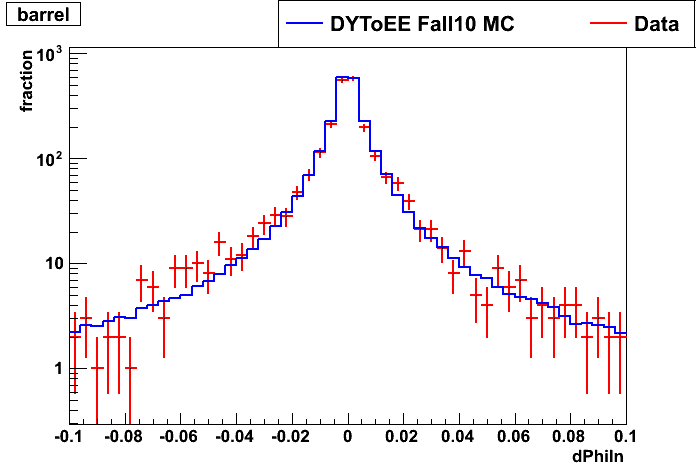
\includegraphics[width=.45\textwidth]{figures/mcdata_dPhiIn_bar_log.png}}
\subfigure[]{
\centering
\label{subfig:mcdata_dEtaIn_bar_log}
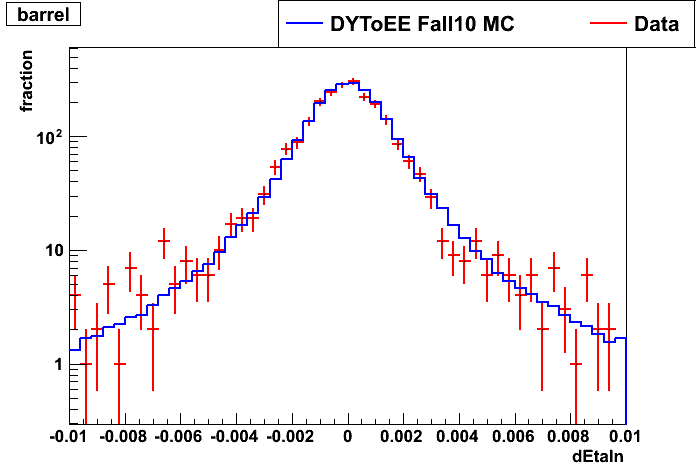
\includegraphics[width=.45\textwidth]{figures/mcdata_dEtaIn_bar_log.png}}\\
\subfigure[]{
\centering
\label{subfig:mcdata_sigmaIEtaIEta_bar_log}
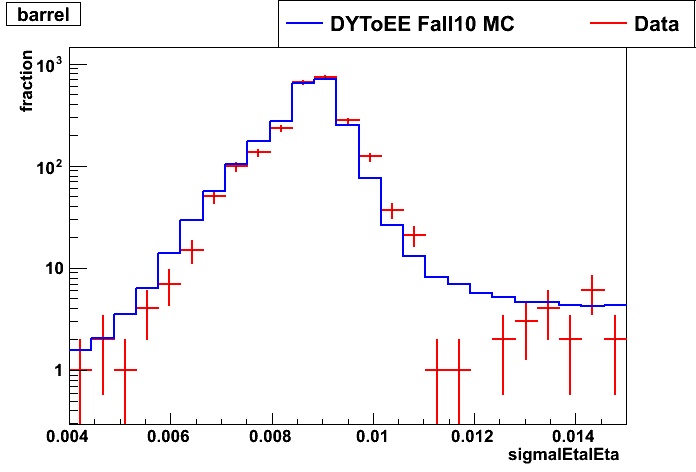
\includegraphics[width=.45\textwidth]{figures/mcdata_sigmaIEtaIEta_bar_log.png}}
\subfigure[]{
\centering
\label{subfig:mcdata_hOverE_bar_log}
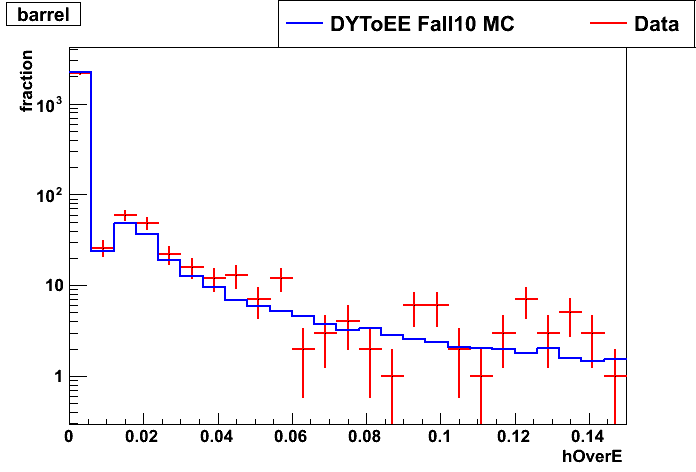
\includegraphics[width=.45\textwidth]{figures/mcdata_hOverE_bar_log.png}}\\
\caption{VBTF electron ID variables (barrel) in MC and in early 2011 data. Distributions are normalized to the number of entries in data.}
\label{fig:mcdata_vbtf_bar}
\end{figure}

\begin{figure}[!hbtp]
\subfigure[]{
\centering
\label{subfig:mcdata_dPhiIn_end_log}
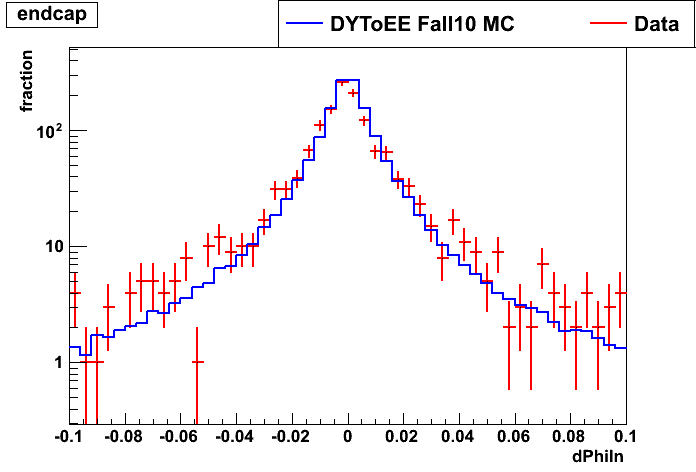
\includegraphics[width=.45\textwidth]{figures/mcdata_dPhiIn_end_log.png}}
\subfigure[]{
\centering
\label{subfig:mcdata_dEtaIn_end_log}
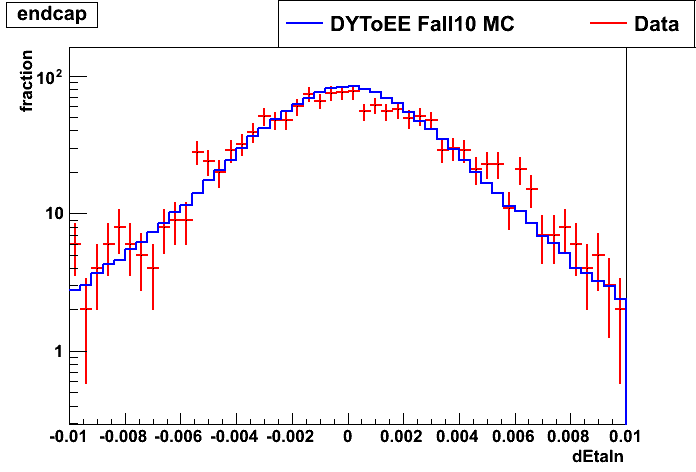
\includegraphics[width=.45\textwidth]{figures/mcdata_dEtaIn_end_log.png}}\\
\subfigure[]{
\centering
\label{subfig:mcdata_sigmaIEtaIEta_end_log}
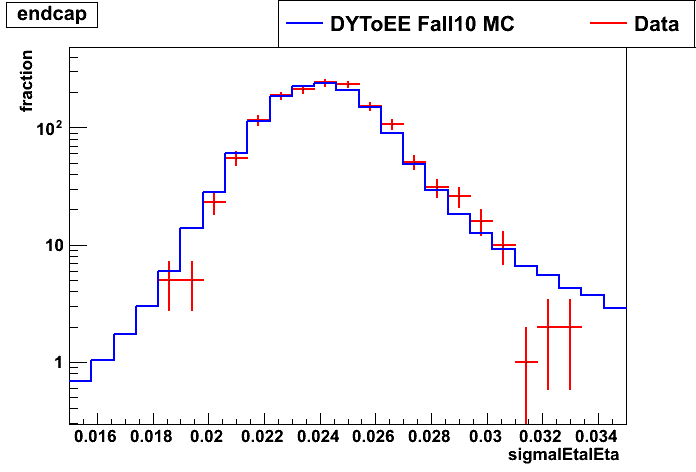
\includegraphics[width=.45\textwidth]{figures/mcdata_sigmaIEtaIEta_end_log.png}}
\subfigure[]{
\centering
\label{subfig:mcdata_hOverE_end_log}
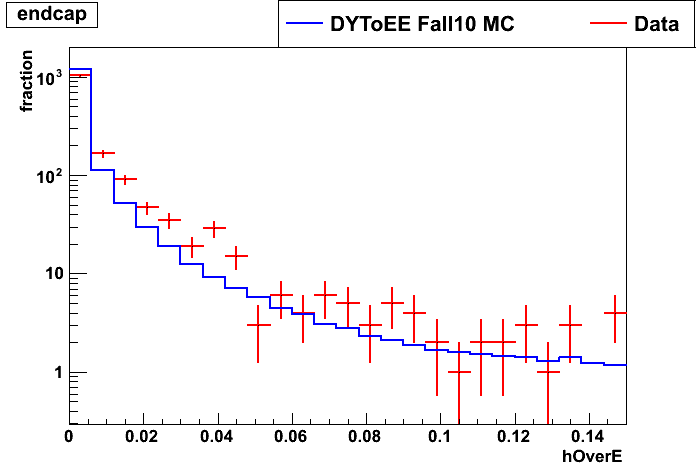
\includegraphics[width=.45\textwidth]{figures/mcdata_hOverE_end_log.png}}\\
\caption{VBTF electron ID variables (endcap) in MC and in early 2011 data. Distributions are normalized to the number of entries in data.}
\label{fig:mcdata_vbtf_end}
\end{figure}


\begin{figure}[!hbtp]
\subfigure[]{
\centering
\label{subfig:mcdata_fbrem_bar1_log}
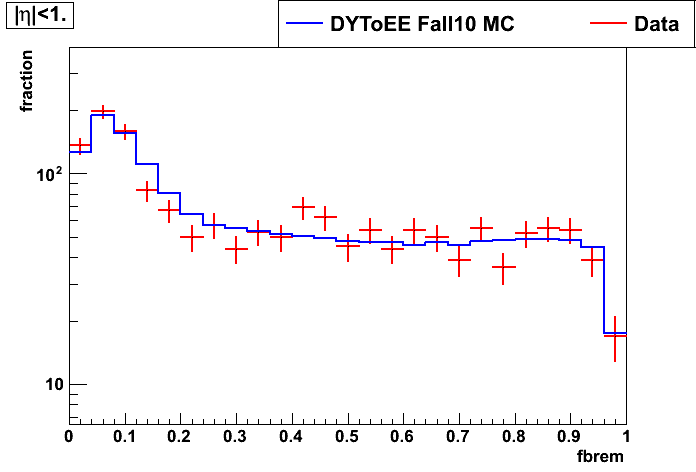
\includegraphics[width=.45\textwidth]{figures/mcdata_fbrem_bar1_log.png}}
\subfigure[]{
\centering
\label{subfig:mcdata_fbrem_end1_log}
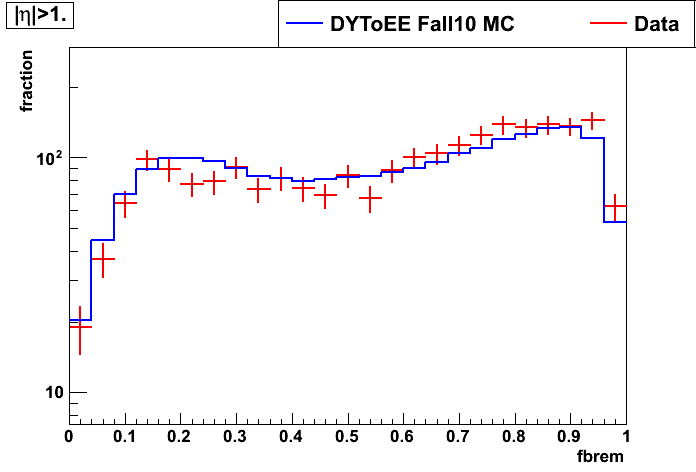
\includegraphics[width=.45\textwidth]{figures/mcdata_fbrem_end1_log.png}}\\
\subfigure[]{
\centering
\label{subfig:mcdata_eOverPIn_bar1_log}
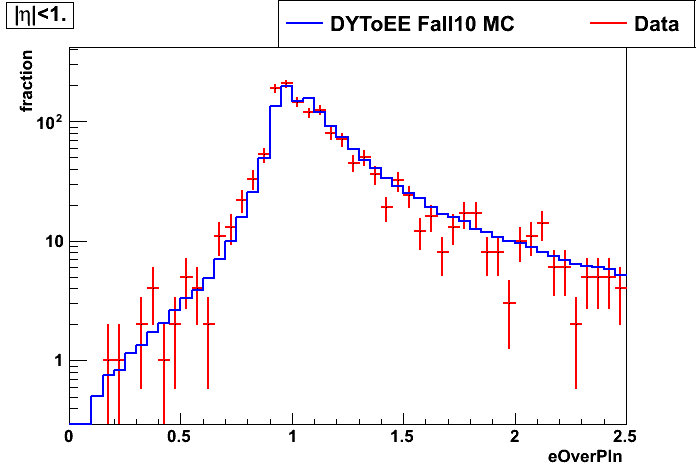
\includegraphics[width=.45\textwidth]{figures/mcdata_eOverPIn_bar1_log.png}}
\caption{VBTF+ additional electron ID variables in MC and in early 2011 data. Distributions are normalized to the number of entries in data.}
\label{fig:mcdata_smurf}
\end{figure}

\begin{figure}[!hbtp]
\subfigure[]{
\centering
\label{subfig:idEffic_15pt20_nohoe}
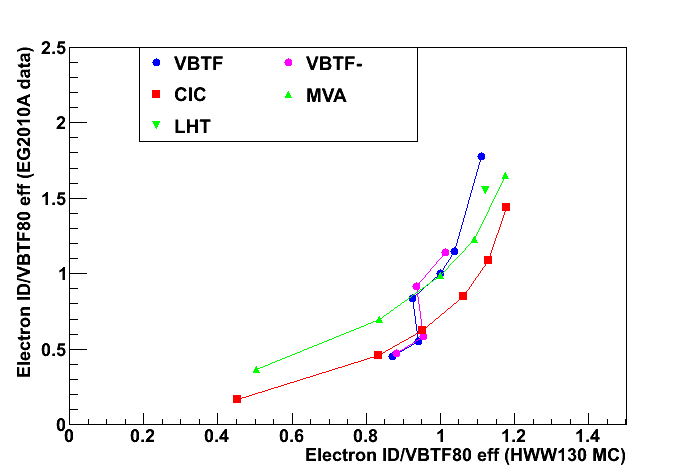
\includegraphics[width=.45\textwidth]{figures/idEffic_15pt20_nohoe.png}}
\subfigure[]{
\centering
\label{subfig:id_hww130_fom1_pt15_nohoe}
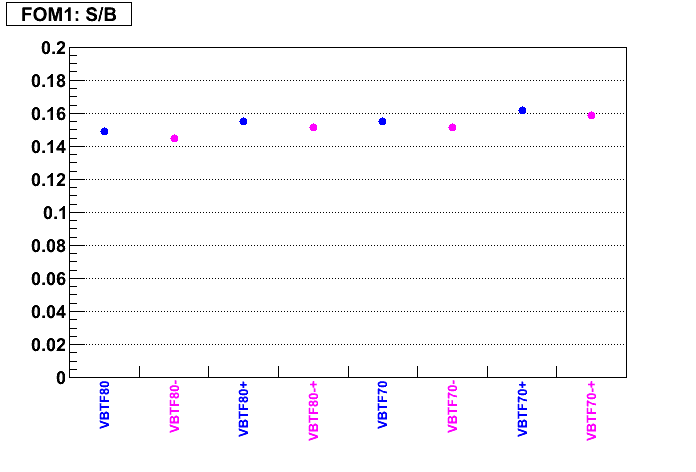
\includegraphics[width=.45\textwidth]{figures/id_hww130_fom1_pt15_nohoe.png}}\\
\subfigure[]{
\centering
\label{subfig:id_hww130_fom2_pt15_nohoe}
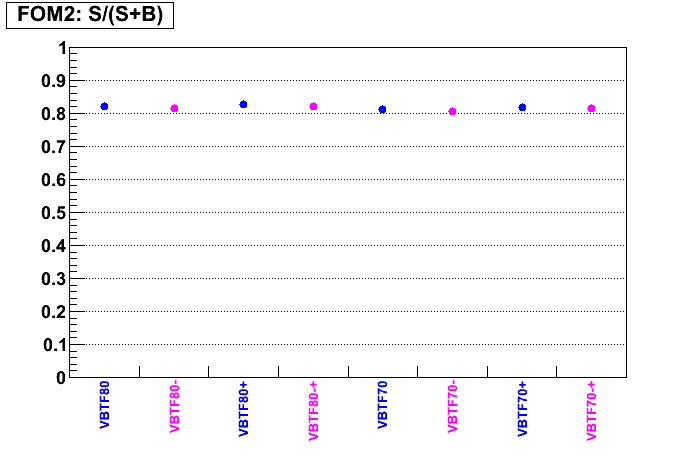
\includegraphics[width=.45\textwidth]{figures/id_hww130_fom2_pt15_nohoe.png}}
\subfigure[]{
\centering
\label{subfig:id_hww130_fom3_pt15_nohoe}
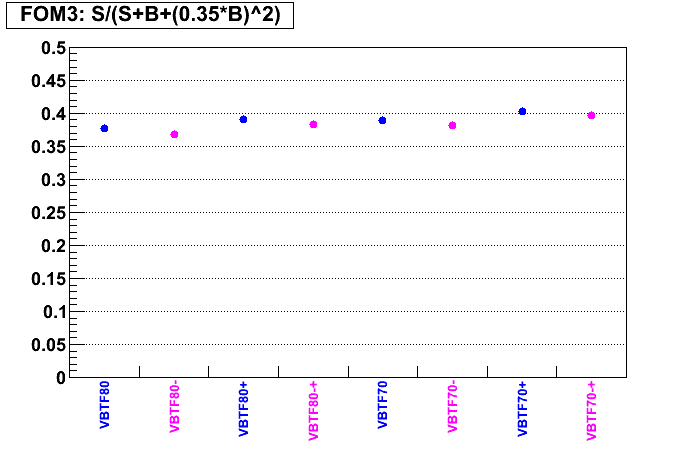
\includegraphics[width=.45\textwidth]{figures/id_hww130_fom3_pt15_nohoe.png}}\\
\caption{Relative ID efficiency for (w.r.t. VBTF80) on fake electrons from data vs good electrons from signal MC including VBTF- \subref{subfig:idEffic_15pt20_nohoe} 
(15$<p_T<$20 GeV);
FOM1, FOM2 and FOM3 \subref{subfig:id_hww130_fom1_pt15_nohoe},\subref{subfig:id_hww130_fom2_pt15_nohoe},\subref{subfig:id_hww130_fom3_pt15_nohoe} for analysis with  
$p_{T,min}>$15 GeV; the 2010 selection is used as a baseline, the ID cut is varied comparing VBTF with VBTF-.}
\label{fig:idpt15_nohoe}
\end{figure}

\subsection{Conclusion}
After the optimization procedure and the tests on data we define the following electron selection for 2011 $H\rightarrow WW$ analysis (conversion rejection not included here, it was optimized with a different procedure):
\begin{itemize}
\item identification: 
  \begin{itemize}
  \item 15$<$pt$<$20: VBTF70 (no H/E cut for endcap) AND (fbrem$>$0.15 OR ($|\eta|<$1 AND E/p$>$0.95)
  \item pt$>$20: VBTF80 (no H/E cut for endcap)
  \end{itemize}
\item isolation: relIso$<$0.10, where relIso is the sum of contributions from tracks, ECAL and HCAL is a cone of R=0.3 around the electron, 
  divided by the electron $p_T$; in the barrel the ECAL contribution has a pedestal subtrction of 1 GeV;
\item impact parameter: transverse longitudinal parameter w.r.t. the primary vertex $<0.02$ cm and longitudinal i.p. $<$ 0.2 cm;
\end{itemize}
